\documentclass[14pt]{beamer}
\usetheme{Warsaw}
\usecolortheme{beaver}
\usefonttheme{professionalfonts}

\input{../../preamble}
\usepackage{amscd,amsmath,amssymb,amsthm,graphicx}
\usepackage[mathscr]{eucal}
\usepackage{paralist}
\usepackage{tabto}
\usepackage[normalem]{ulem}
\usepackage{tikz}
\usepackage{tkz-euclide}
\usetkzobj{all}

% % % % % % % % % %
\title[Cal I S2015]{MATH 2554 (Calculus I)}
\subtitle{}
\author[Wheeler]{Dr. Ashley K. Wheeler}
\institute{University of Arkansas}
\date{\today}
\logo{}

% % %
\begin{document}
\maketitle

% % %
\begin{frame}
\frametitle{Table of Contents}
\tableofcontents
\end{frame}

% % % % % % % % % % Mon 9 Mar 2015

% % %
\begin{frame}
\section[Week 9]{Week 9: 9-13 March}
\frametitle{Monday 9 March (Week 9)}
\small
\begin{itemize}
\item computer HW for $\oint 3.8-3.9$ is extended to Wednesday night
\item midterm returned in drill
\item Quiz \#7 on Tues 10 Mar -- covers $\oint 3.8-3.9$	
\item sub on Friday: Dr. Paulk
\end{itemize}
\end{frame}

% % %
\begin{frame}
\frametitle{CEA REQUEST}
\footnotesize {\bf
A student in this class requires a note-taker. If you are willing to upload your notes and plan to attend class on a REGULAR basis, please sign up via the CEA Online Services on the Center for Educational Access (CEA) website http://cea.uark.edu. On the CEA Online Services login screen, click on ``Sign Up as a Note-taker". At the end of the semester you will receive verification of 48 community service hours OR a \$50 gift card for providing class notes. All interested students are encouraged to sign up; preference may be given to volunteers seeking community service in an effort engage U of A students in community service opportunities. Please contact the Center for Educational Access at ceanotes@uark.edu if you have any questions.}
\end{frame}

% % %
\begin{frame}
\subsection[$\oint 3.8$, cont.]{$\oint 3.8$, cont.}
\frametitle{\small $\oint 3.8$, cont.}
\footnotesize
The relationship $y=\ln x \Longleftrightarrow x=e^y$ applies to logarithms of other bases:
\[y=\log_b x \quad\Longleftrightarrow\quad x=b^y.\]
Now taking $\dfrac{d}{dx}\left(x=b^y\right)$ we obtain
\vspace{-0.75pc}
\begin{align*}
1 &= b^y\ln b\left(\frac{dy}{dx}\right) \\
\frac{dy}{dx} &= \frac{1}{b^y \ln b} \\[0.5pc]
 &=\frac{1}{x \ln b}
\end{align*}
\bigskip
So \alert{$\dfrac{d}{dx}(\log_b x)=\dfrac{1}{x \ln b}$}.
\end{frame}

% % %
\begin{frame}
\frametitle{\small Neat Trick: Logarithmic Differentiation}
\begin{ex}  Compute the derivative of $f(x)=\dfrac{x^2(x-1)^3}{(3+5x)^4}$. \end{ex}

We can use logarithmic differentiation: first take the natural log of both sides and then use properties of logarithms.
\end{frame}

% % %
\begin{frame}
\small
\begin{alignat*}{2}
\ln(f(x)) &= \ln \left( \dfrac{x^2(x-1)^3}{(3+5x)^4} \right) \\[0.5pc]
&= \ln{x^2} + \ln{(x-1)^3}-\ln{(3+5x)^4} \\[0.5pc]
&= 2\ln x + 3\ln(x-1)-4\ln(3+5x)
\end{alignat*}
\alert{Now} we take $\dfrac{d}{dx}$ on both sides:
\begin{alignat*}{2}
\dfrac{1}{f(x)}\left(\dfrac{df}{dx}\right) &= 2\left(\frac{1}{x}\right) + 3\left(\frac{1}{x-1}\right) - 4\left(\frac{1}{3+5x}\right)(5) \\[1pc]
\dfrac{f^{\prime}(x)}{f(x)} &= \dfrac{2}{x} + \dfrac{3}{x-1} - \dfrac{20}{3+5x}
\end{alignat*}
\end{frame}

% % %
\begin{frame}
\frametitle{}
Finally, solve for $f^{\prime}(x)$:
\begin{alignat*}{2}
f^{\prime}(x) &= \alert{f(x)} \left[ \dfrac{2}{x} + \dfrac{3}{x-1} - \dfrac{20}{3+5x} \right] \\[1pc]
&= \alert{\frac{x^2 (x-1)^3}{(3+5x)^4}} \left[ \dfrac{2}{x} + \dfrac{3}{x-1} - \dfrac{20}{3+5x} \right]
\end{alignat*}
\end{frame}

% % %
\begin{frame}
\frametitle{HW from Section 3.8}
Do problems 9--27 odd, 31--37 odd, 41--47 odd (pp.\ 199--200 in textbook)
\end{frame}

% % %
\begin{frame}
\subsection[$\oint 3.9$ Derivatives of Inverse Trigonometric Functions]{$\oint 3.9$ Derivatives of Inverse Trigonometric Functions}
\frametitle{\small $\oint 3.9$ Derivatives of Inverse Trigonometric Functions}
\small 
{\bf Recall:} If $y=f(x)$, then $f^{-1}(x)$ is the value of $y$ such that $x=f(y)$.

\vspace{1pc}
\begin{ex} If $f(x)=3x+2$, then what is $f^{-1}(x)$? \end{ex}

\vspace{2pc}
{\bf NOTE:}  $f^{-1}(x)\alert{\neq} f(x)^{-1}\left(=\dfrac{1}{f(x)}\right)$
\end{frame}

% % %
\begin{frame}
\frametitle{\small Derivative of Inverse Sine}
\footnotesize
{\bf Remember,} trig functions are functions, too.  Just like with ``$f\,$", there has to be something to ``plug in".  It makes no sense to just say $\sin$, without having $\sin(\text{\alert{\it something}})$.
\[y=\sin^{-1}x \Longleftrightarrow x=\sin y\]  

The derivative of $y=\sin^{-1}x$ can be found using implicit differentiation: 
\begin{alignat*}{2}
x &= \sin y \\
\frac{d}{dx}(x) &= \frac{d}{dx}(\sin y) \\
1 &= (\cos y) \frac{dy}{dx} \\
\frac{dy}{dx} &= \frac{1}{\cos y}
\end{alignat*}
\end{frame}

% % %
\begin{frame}
\frametitle{}
\footnotesize
We still need to replace $\cos y$ with an expression in terms of $x$.  We use the trig identity $\sin^2 y + \cos^2 y = 1$ (careful with notation: in this case we mean $\left(\sin y\right)^2+\left(\cos y\right)^2=1$).  Then 
\[\cos y= \pm \sqrt{1-\sin^2 y}=\pm\sqrt{1-x^2}.\]

The range of $y=\sin^{-1}x$ is $-\frac{\pi}{2} \leq y \leq \frac{\pi}{2}$.  In this range, cosine is never negative, so we can just take the positive portion of the square root.

\vspace{1pc}
Therefore,
\[\frac{dy}{dx}=\frac{1}{\cos y}=\frac{1}{\sqrt{1-x^2}} \implies \alert{\frac{d}{dx}(\sin^{-1}x)=\frac{1}{\sqrt{1-x^2}}}.\]
\end{frame}

% % %
\begin{frame}
\frametitle{}
\begin{exe} Compute the following:

\vspace{0.5pc}
\begin{itemize}
\item[1.] $\dfrac{d}{dx} \left( \sin^{-1}(4x^2-3) \right)$

\vspace{1pc}
\item[2.] $\dfrac{d}{dx} \left( \cos(\sin^{-1}x) \right)$
\end{itemize}
\end{exe}
\end{frame}

% % %
\begin{frame}
\frametitle{\small Derivative of Inverse Tangent}
\footnotesize
We use a similar method as with inverse sine.  Let $y=\tan^{-1}x$ and use implicit differentiation:
\vspace{-0.5pc}
\begin{alignat*}{2}
x &= \tan y \\
\frac{d}{dx}(x) &= \frac{d}{dx} (\tan y) \\
1 &= (\sec^2 y) \frac{dy}{dx} \\
\frac{dy}{dx} &= \frac{1}{\sec^2 y}
\end{alignat*}

\vspace{1pc}
Use the trig identity $\sec^2 y-\alert{\tan^2 y}=1$ to replace $\sec^2 y$ with $1+\alert{x^2}$:
\[\frac{d}{dx}(\tan^{-1} x)=\frac{1}{1+x^2}\]
\end{frame}

% % %
\begin{frame}
\frametitle{\small Derivative of Inverse Secant}
\footnotesize
Again, use the same method as with inverse sine:
\begin{alignat*}{2}
y &= \sec^{-1}x \\
x &= \sec y \\
\frac{d}{dx}(x) &= \frac{d}{dx} (\sec y) \\
1 &= \sec y \tan y \frac{dy}{dx} \\
\frac{dy}{dx} &= \frac{1}{\sec y \tan y}
\end{alignat*}
Use the trig identity $\sec^2 y-\tan^2 y=1$ again to get 
\[\tan y=\pm\sqrt{\sec^2 y-1}=\pm\sqrt{x^2-1}.\]
\end{frame}

% % %
\begin{frame}
\frametitle{}
\footnotesize
This time, the $\pm$ matters:

\vspace{0.25pc}
\centering{\includegraphics[width=0.75\textwidth]{invSecpic}}
\begin{itemize}
\item If $x \ge 1$, then $0\le y<\dfrac{\pi}{2}$ and so $\tan y >0.$  

\vspace{-0.5pc}
\item If $x \le -1$, then $\dfrac{\pi}{2} < y \le \pi$ and so  $\tan y <0$.  
\end{itemize}
\end{frame}

% % %
\begin{frame}
\frametitle{}
\small
Therefore,
\[\frac{d}{dx}(\sec^{-1} x)=\frac{1}{|x|\sqrt{x^2-1}}.\]

\vspace{1pc}
\hrulefill

\vspace{1pc}
\footnotesize
Using other trig identities (which you do not need to prove)
%\vspace{-0.5pc}
\[\cos^{-1}x+\sin^{-1}x=\dfrac{\pi}{2}\quad \cot^{-1}x+\tan^{-1}x=\dfrac{\pi}{2}\quad \csc^{-1}x+\sec^{-1}x=\dfrac{\pi}{2}\] 

%\vspace{-0.5pc}
we can get the rest of the inverse trig derivatives. 
\end{frame}

% % %
\begin{frame}
\frametitle{\small All other inverse trig derivatives}
To summarize:
\begin{columns}%[T]
\begin{column}{0.45\textwidth}
%\begin{block}
\begin{itemize}
\footnotesize
\item[]$\frac{d}{dx}(\sin^{-1}x)=\frac{1}{\sqrt{1-x^2}}$ \vspace{1pc}
\item[]$\frac{d}{dx}(\tan^{-1}x)=\frac{1}{1+x^2}$ \vspace{1pc}
\item[]$\frac{d}{dx}(\sec^{-1}x)=\frac{1}{|x|\sqrt{x^2-1}}$ 
\end{itemize}
%\end{block}
\end{column}

\begin{column}{0.6\textwidth}
%\begin{block}
\begin{itemize}
\footnotesize
\item[] $\frac{d}{dx}(\cos^{-1}x)=-\frac{1}{\sqrt{1-x^2}}$ \\[0.25pc] $\quad (-1<x<1)$ \vspace{1pc}
\item[] $\frac{d}{dx}(\cot^{-1}x)=-\frac{1}{1+x^2}$ \\[0.25pc] $\quad (-\infty<x<\infty) $ \vspace{1pc}
\item[] $\frac{d}{dx}(\csc^{-1}x)=-\frac{1}{|x|\sqrt{x^2-1}}$ \\[0.25pc] $\quad (|x|>1)$ 
\end{itemize}
%\end{block}
\end{column}
\end{columns}
\end{frame}

% % %
\begin{frame}
\frametitle{}
\begin{ex} Compute the derivatives of $f(x)=\tan^{-1}\left(\frac{1}{x}\right)$ and $g(x)=\sin \left(\sec^{-1}(2x) \right)$. \end{ex}
\end{frame}

% % %
\begin{frame}[t]
\frametitle{\small Derivatives of Inverse Functions in General}
\small
Let $f$ be differentiable and have an inverse on an interval $I$.  Let $x_0$ be a point in $I$ at which $f^{\prime}(x_0)\ne0$.

Then $f^{-1}$ is differentiable at $y_0=f(x_0)$ and 
$$\left(f^{-1}\right)^{\prime}(y_0)=\frac{1}{f^{\prime}(x_0)}$$
where $y_0=f(x_0).$

\begin{ex} Let $f(x)=\dfrac{1}{4}x^3+x-1$.  Find $\left(f^{-1}\right)^{\prime}(3)$. \end{ex}
\end{frame}

% % %
\begin{frame}
\frametitle{HW from Section 3.9}
Do problems 7--27 odd, 31--39 odd.
\end{frame}

% % % % % % % % % % Wed 11 Mar 2015

% % %
\begin{frame}
\frametitle{Wednesday 11 March (Week 9)}
\small
\begin{itemize}
\item computer HW for $\oint 3.8-3.9$ is extended to tonight
\item sub on Friday: Dr. Paulk
\item midterm returned in drill... 
\item Quiz schedule: 
	\begin{itemize}
	\small 
	\item Quiz \#8: $\oint 3.10$ Thurs 12 Mar, take-home
	\item Quiz \#9: $\oint 4.1,4.2$ Thurs 19 Mar, due upon return from spring break
	\item Quiz \#10: $\oint 4.4$ in class Tues 31 Mar
	\end{itemize}
\item Exam \#3: Friday 3 April	
\end{itemize}
\end{frame}

% % %
\begin{frame}
\frametitle{CEA REQUEST}
\footnotesize {\bf
A student in this class requires a note-taker. If you are willing to upload your notes and plan to attend class on a REGULAR basis, please sign up via the CEA Online Services on the Center for Educational Access (CEA) website http://cea.uark.edu. On the CEA Online Services login screen, click on ``Sign Up as a Note-taker". At the end of the semester you will receive verification of 48 community service hours OR a \$50 gift card for providing class notes. All interested students are encouraged to sign up; preference may be given to volunteers seeking community service in an effort engage U of A students in community service opportunities. Please contact the Center for Educational Access at ceanotes@uark.edu if you have any questions.}
\end{frame}

% % %
\begin{frame}
\subsection[$\oint 3.10$ Related Rates]{$\oint 3.10$ Related Rates}
\frametitle{$\oint 3.10$ Related Rates}
\small 
In this section, we use our knowledge of derivatives to examine how variables change with respect to time.

\vspace{1pc}
The prime feature of these problems is that two or more variables, which are related in a known way, are themselves changing in time.

\vspace{1pc}
The goal of these types of problems is to determine the rate of change (i.e., the derivative) of one or more variables at a specific moment in time.
\end{frame}

% % %
\begin{frame}
\frametitle{}
\begin{block}{Problem}
The edges of a cube increase at a rate of 2 cm/sec.  How fast is the volume changing when the length of each edge is 50 cm?
\end{block}
\small
\begin{itemize}
\item {\bf Variables:}  $V$ (Volume of the cube) and $x$ (length of edge)
\item {\bf How Variables are related:}  $V=x^3$
\item {\bf Rates Known:}  $\dfrac{dx}{dt}=2\ \text{cm/sec}$
\item {\bf Rate We Seek:}  $\dfrac{dV}{dt}$ when $x=50\ \text{cm}$
\end{itemize}
\end{frame}

% % % 
\begin{frame}
\small
Note that both $V$ and $x$ are functions of $t$ (their respective sizes are dependent upon how much time has passed).

\vspace{1pc}
So we can write $V(t)=x(t)^3$ and then differentiate this with respect to $t$:
$$V^{\prime}(t) = 3 x(t)^2 \cdot x^{\prime}(t).$$

\vspace{1pc}
{\bf Note that $x(t)$ is the length of the cube's edges at time $t$, and $x^{\prime}(t)$ is the rate at which the edges are changing at time $t$.}
\end{frame}

% % %
\begin{frame}

We can rewrite the previous equation as

\[\frac{dV}{dt}=3x^2 \cdot \frac{dx}{dt}.\]

\vspace{1pc}
So the rate of change of the volume when $x=50\ \text{cm}$ is 
\[\left.\frac{dV}{dt}\right|_{x=50}=3\cdot 50^2 \cdot 2 = 15000\ \text{cm}^3/\text{sec}.\]
\end{frame}

% % %
\begin{frame}
\frametitle{\small Steps for Solving Related Rates Problems}
\small
\begin{itemize}
\item[1.] Read the problem carefully, making a sketch to organize the given information.  Identify the rates that are given and the rate that is to be determined.
\item[2.] Write one or more equations that express the basic relationships among the variables.
\item[3.] Introduce rates of change by differentiating the appropriate equation(s) with respect to time $t$.
\item[4.] Substitute known values and solve for the desired quantity.
\item[5.] Check that the units are consistent and the answer is reasonable.
\end{itemize}
\end{frame}

% % %
\begin{frame}
\frametitle{}
\begin{block}{The Jet Problem}
A jet ascends at a $10^{\circ}$ angle from the horizontal with an airspeed of 550 miles/hr (its speed along its line of flight is 550 miles/hr).  How fast is the altitude of the jet increasing?  If the sun is directly overhead, how fast is the shadow of the jet moving on the ground?
\end{block}
\end{frame}

% % %
\begin{frame}
\small
{\bf Step 1:}  There are three variables:  the distance the shadow has traveled ($x$), the altitude of the jet ($h$), and the distance the jet has actually traveled on its line of flight ($z$).  We know that $\dfrac{dz}{dt}=550\ \text{miles/hr}$ and we want to find $\dfrac{dx}{dt}$ and $\dfrac{dh}{dt}$.  We also see that these variables are related through a right triangle:
\begin{center}
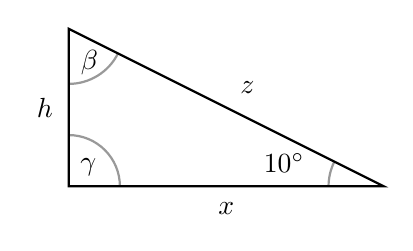
\begin{tikzpicture}[thick]
\coordinate (O) at (0,0);
\coordinate (A) at (4,0);
\coordinate (B) at (0,2);
\draw (O)--(A)--(B)--cycle;
\tkzLabelSegment[below=2pt](O,A){$x$}
\tkzLabelSegment[left=2pt](O,B){$h$}
\tkzLabelSegment[above right=2pt](A,B){$z$}
\tkzMarkAngle[fill= orange,size=0.65cm,opacity=.4](A,O,B)
\tkzLabelAngle[pos = 0.35](A,O,B){$\gamma$}
\tkzMarkAngle[size=0.7cm,opacity=.4](B,A,O)
\tkzLabelAngle[pos = 1.3](B,A,O){$10^{\circ}$}
\tkzMarkAngle[fill= orange,size=0.7cm,opacity=.4](O,B,A)
\tkzLabelAngle[pos = 0.5](O,B,A){$\beta$}
\end{tikzpicture}
\end{center}
\end{frame}

% % %
\begin{frame}
\small
{\bf Step 2:}  To answer how fast the altitude is increasing, we need an equation involving only $h$ and $z$.  Using trigonometry,
\[\sin(10^{\circ})=\frac{h}{z} \implies h=\sin(10^{\circ}) \cdot z.\]

\vspace{1pc}
To answer how fast the shadow is moving, we need an equation involving only $x$ and $z$.  Using trigonometry,
\[\cos(10^{\circ})=\frac{x}{z} \implies x=\cos(10^{\circ}) \cdot z.\]
\end{frame}

% % %
\begin{frame}
\footnotesize
{\bf Step 3:}  We can now differentiate each equation to answer each question:
\begin{alignat*}{2}
h=\sin(10^{\circ}) \cdot z &\implies \dfrac{dh}{dt}=\sin(10^{\circ}) \dfrac{dz}{dt} \\
x=\cos(10^{\circ}) \cdot z &\implies \dfrac{dx}{dt}=\cos(10^{\circ}) \dfrac{dz}{dt}
\end{alignat*}

\vspace{1pc}
{\bf Step 4:}  We know that $\dfrac{dz}{dt}=550\ \text{miles/hr}$.  So 
\begin{alignat*}{2}
\dfrac{dh}{dt} &=\sin(10^{\circ}) \cdot 550 \approx 95.5\ \text{miles/hr}\\
\dfrac{dx}{dt} &=\cos(10^{\circ}) \cdot 550 \approx 541.6\ \text{miles/hr}
\end{alignat*}
\end{frame}

% % %
\begin{frame}
\frametitle{}
{\bf Step 5:}  Because both answers are in terms of miles/hr and both answers seem reasonable within the context of the problem, we conclude that the jet is gaining altitude at a rate of 95.5 miles/hr, while the shadow on the ground is moving at about 541.6 miles/hr.
\end{frame}

% % %
\begin{frame}%[t]
\frametitle{}
\begin{ex} The sides of a cube increase at a rate of $R$ cm/sec.  When the sides have a length of 2 cm, what is the rate of change of the volume? \end{ex}
\end{frame}

% % %
\begin{frame}%[t]
\frametitle{}
\begin{ex} Two boats leave a dock at the same time.  One boat travels south at 30 miles/hr and the other travels east at 40 miles/hr.  After half an hour, how fast is the distance between the boats increasing? \end{ex}
\end{frame}

% % %
\begin{frame}
\frametitle{HW for Section 3.10}
Do problems 5--12 all, 14--15, 17--18, 30--31.
\end{frame}

% % %
\begin{frame}
\subsection[$\oint 4.1$ Maxima and Minima]{$\oint 4.1$ Maxima and Minima}
\frametitle{$\oint 4.1$ Maxima and Minima}
\small 
\begin{dfn} Let $f$ be defined on an interval $I$ containing $c$.
\begin{itemize}
\item $f$ has an {\bf absolute maximum} value on $I$ at $c$ means $f(c)\ge f(x)$ for every $x$ in $I$.
\item $f$ has an {\bf absolute minimum} value on $I$ at $c$ means $f(c)\le f(x)$ for every $x$ in $I$.
\end{itemize}
\end{dfn}
\end{frame}

% % %
\begin{frame}
\footnotesize
The existence and location of absolute extreme values depend on the function and the interval of interest:
\begin{columns}[T]
\begin{column}{.5\textwidth}
\begin{block}{}
\centering{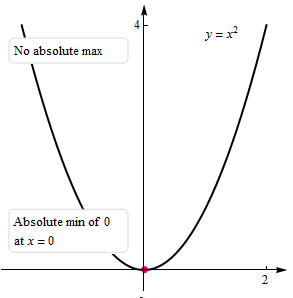
\includegraphics[scale=0.65]{Fig4_2a}}
\end{block}
\end{column}
\begin{column}{.5\textwidth}
\begin{block}{}
\centering{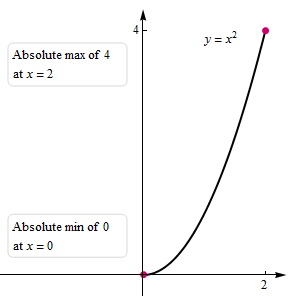
\includegraphics[scale=0.65]{Fig4_2b}}
\end{block}
\end{column}
\end{columns}
\end{frame}

% % %
\begin{frame}
\frametitle{}
\begin{columns}%[T]
\begin{column}{.5\textwidth}
\begin{block}{}
\centering{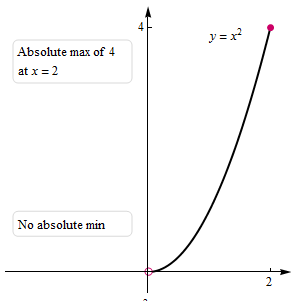
\includegraphics[scale=0.65]{Fig4_2c}}
\end{block}
\end{column}
\begin{column}{.5\textwidth}
\begin{block}{}
\centering{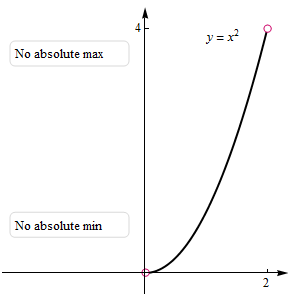
\includegraphics[scale=0.65]{Fig4_2d}}
\end{block}
\end{column}
\end{columns}
\end{frame}

% % %
\begin{frame}
\frametitle{Extreme Value Theorem}
\small
\begin{thm}[Extreme Value Theorem] A function that is continuous on a closed interval $[a,b]$ has an absolute maximum value and an absolute minimum value on that interval. \end{thm}

\vspace{1pc}
The EVT provides the criteria that ensures absolute extrema:
\begin{itemize}
\item the function must be continuous on the interval of interest;
\item the interval of interest must be closed and bounded.
\end{itemize}
\end{frame}

% % %
\begin{frame}
\frametitle{Local Maxima and Minima}
\small
Beyond absolute extrema, a graph may have a number of peaks and dips throughout its interval of interest:
\begin{center}
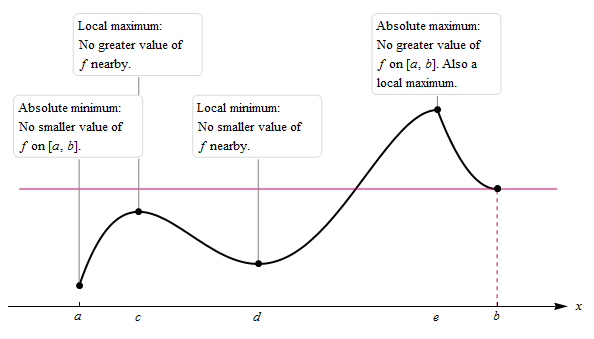
\includegraphics[scale=0.625]{Fig4_5}
\end{center}
\end{frame}

% % %
\begin{frame}
\frametitle{}
\small
\begin{dfn} Suppose $I$ is an interval on which $f$ is defined and $c$ is an interior point of $I$.
\begin{itemize}
\item If $f(c)\ge f(x)$ for all $x$ in some open interval containing $c$, then $f(c)$ is a {\bf local maximum} value of $f$.
\item If $f(c)\le f(x)$ for all $x$ in some open interval containing $c$, then $f(c)$ is a {\bf local minimum} value of $f$.
\end{itemize}
\end{dfn}
\end{frame}

% % %
\begin{frame}
\frametitle{}
\small
\begin{exe} Use the graph below to identify the points on the interval $[a,b]$ at which local and absolute extreme values occur.
\begin{center}
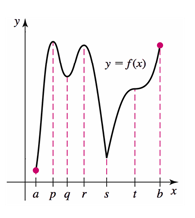
\includegraphics[scale=0.9]{Ch4Sect1_Prob16}
\end{center}
\end{exe}
\end{frame}

% % %
\begin{frame}
\frametitle{Critical Points}
Based on the previous graph, how is the derivative related to where the local extrema occur?

\vspace{1pc}
Local extrema occur where the derivative either does not exist or is equal to 0.

\begin{dfn} An interior point $c$ of the domain of $f$ at which $f^{\prime}(c)=0$ or $f^{\prime}(c)$ fails to exist is called a {\bf critical point} of $f$. \end{dfn}
\end{frame}

% % %
\begin{frame}
\frametitle{Local Extreme Point Theorem}
\small
\begin{thm}[Local Extreme Point Theorem] If $f$ has a local minimum or maximum value at $c$ and $f^{\prime}(c)$ exists, then $f^{\prime}(c)=0$.  \alert{\bf (Converse is not true!)} \end{thm}

It is possible for $f^{\prime}(c)=0$ or $f^{\prime}(c)$ not to exist at a point, yet the point not be a local min or max.  Therefore, critical points provide {\bf candidates} for local extrema, but do not guarantee that the points are local extrema (see p.\ 227 immediately before Figure 4.9 for examples).
\end{frame}

% % %
\begin{frame}
\frametitle{Locating Absolute Min and Max}
%\small
Two facts help us in the search for absolute extrema:

\begin{itemize}
\item Absolute extrema in the interior of an interval are also local extrema, which occur at critical points of $f$.
\item Absolute extrema may occur at the endpoints of $f$.
\end{itemize}
\end{frame}

% % %
\begin{frame}
\frametitle{}
\footnotesize
{\bf Procedure: } Assume that the function $f$ is continuous on $[a,b]$.

\begin{itemize}
\item[1.] Locate the critical points $c$ in $(a,b)$, where $f^{\prime}(c)=0$ or $f^{\prime}(c)$ does not exist.  These points are {\bf candidates} for absolute extrema.
\item[2.] Evaluate $f$ at the critical points and at the endpoints of $[a,b]$.
\item[3.] Choose the largest and smallest values of $f$ from Step 2 for the absolute max and min values, respectively.
\end{itemize}

NOTE:  In this section, given an equation, we can identify critical points and absolute extrema, \alert{BUT NOT LOCAL EXTREMA}.  Techniques for locating local extrema come in later sections.
\end{frame}

% % %
\begin{frame}%[t]
\frametitle{}
\begin{exe} Given $f(x)=(x+1)^{4/3}$ on $[-8,8]$, determine the critical points and the absolute extreme values of $f$. \end{exe}
\end{frame}

% % %
\begin{frame}
\frametitle{HW for Section 4.1}
Do problems 11--25 odd, 31--45 odd (pp.\ 229--230 in textbook)
\end{frame}

\begin{comment}
\end{comment}

\end{document}